\documentclass[border=3pt]{standalone}
% Preâmbulo compartilhado pelos diagramas TikZ da aula 4 de Navegação (Representação de Mapas)
\usepackage[T1]{fontenc}
\usepackage[utf8]{inputenc}
\usepackage{lmodern}
\usepackage{amsmath}
\usepackage{xcolor}
\usepackage{tikz}
\usetikzlibrary{arrows.meta,angles,quotes,decorations.pathmorphing,decorations.pathreplacing,calc,
                positioning,shapes.geometric,shapes.misc,backgrounds,fit,
                math}

% Paleta (mesma dos SVGs originais)
\definecolor{dblue}{HTML}{2A5B8C}
\definecolor{dorange}{HTML}{B3541E}
\definecolor{dgreen}{HTML}{4A7C59}
\definecolor{dred}{HTML}{9C4B4B}
\definecolor{dcream}{HTML}{F4F1EA}
\definecolor{dshade}{HTML}{DDD7C9}

% Função gaussiana (não normalizada por padrão de escala visual)
\pgfmathdeclarefunction{gauss}{3}{%
  \pgfmathparse{1/(#3*sqrt(2*pi))*exp(-((#1-#2)^2)/(2*#3^2))}%
}

% Estilos comuns (prefixo d... para não colidir com chaves internas do pgf)
\tikzset{
  >={Stealth[length=2mm]},
  dguide/.style={gray!55, dashed, line width=0.4pt},
  daxis/.style={gray!60, line width=0.7pt, ->},
  dbody/.style={fill=black!3, draw=black!80, line width=1pt},
  dacc/.style={draw=dblue, line width=1pt},
  dlbl/.style={black!55, font=\small},
  dsub/.style={black!45, font=\footnotesize},
  dstate/.style={circle, draw=black!80, fill=dcream, line width=1pt,
                 minimum size=17mm, font=\large, inner sep=1pt},
  dobs/.style={circle, draw=black!80, fill=dshade, line width=1pt,
               minimum size=14mm, font=\large, inner sep=1pt},
  dbox/.style={rounded corners=2pt, draw=black!80, fill=dcream, line width=1pt,
               align=center, inner sep=6pt},
  dop/.style={circle, draw=black!80, fill=white, line width=1pt,
              minimum size=6mm, inner sep=0pt, font=\small},
  dtrans/.style={->, dblue, line width=1pt},
  dmeas/.style={->, dorange, line width=1pt},
  dcurve/.style={line width=1pt, dblue},
  dcurveb/.style={line width=1.4pt, dorange},
}

\begin{document}
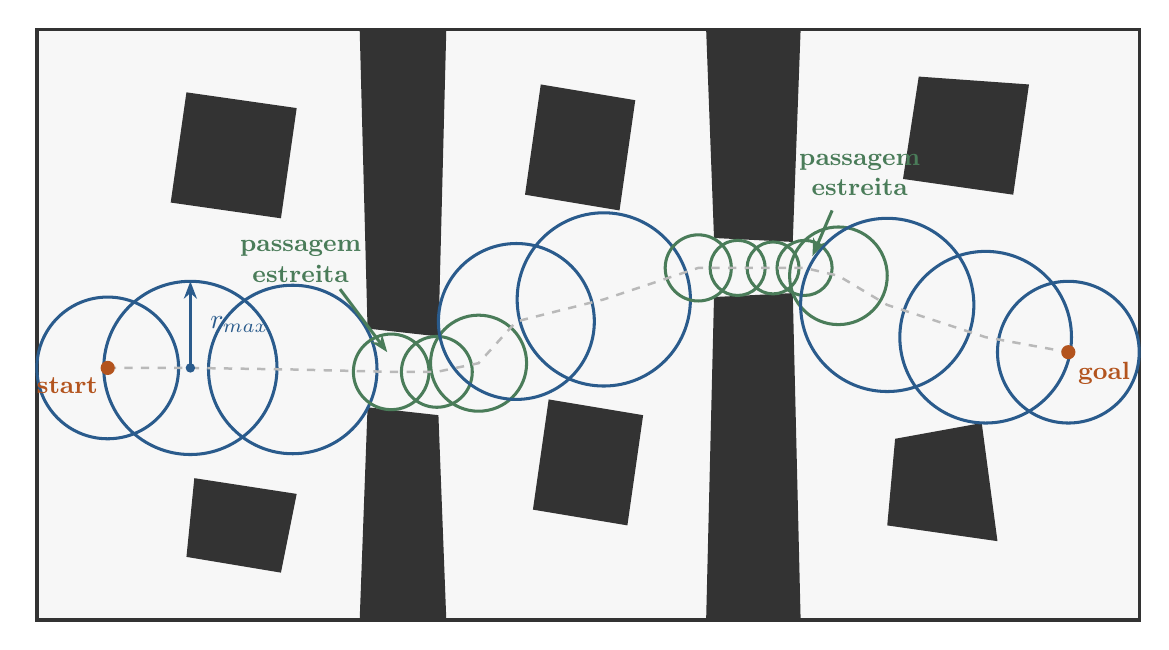
\begin{tikzpicture}[x=1cm,y=1cm]

  \draw[dbody, line width=1.2pt] (0,0) rectangle (14,7.5);

  \fill[black!80] (4.20,3.70) -- (5.10,3.60) -- (5.20,7.50) -- (4.10,7.50) -- cycle;
  \fill[black!80] (4.10,0.00) -- (5.20,0.00) -- (5.10,2.60) -- (4.20,2.70) -- cycle;
  \fill[black!80] (8.60,4.85) -- (9.60,4.80) -- (9.70,7.50) -- (8.50,7.50) -- cycle;
  \fill[black!80] (8.50,0.00) -- (9.70,0.00) -- (9.60,4.15) -- (8.60,4.10) -- cycle;
  \fill[black!80] (1.70,5.30) -- (3.10,5.10) -- (3.30,6.50) -- (1.90,6.70) -- cycle;
  \fill[black!80] (1.90,0.80) -- (3.10,0.60) -- (3.30,1.60) -- (2.00,1.80) -- cycle;
  \fill[black!80] (6.30,1.40) -- (7.50,1.20) -- (7.70,2.60) -- (6.50,2.80) -- cycle;
  \fill[black!80] (6.20,5.40) -- (7.40,5.20) -- (7.60,6.60) -- (6.40,6.80) -- cycle;
  \fill[black!80] (10.80,1.20) -- (12.20,1.00) -- (12.00,2.50) -- (10.90,2.30) -- cycle;
  \fill[black!80] (11.00,5.60) -- (12.40,5.40) -- (12.60,6.80) -- (11.20,6.90) -- cycle;

  \draw[dblue, line width=1.1pt] (0.90,3.20) circle (0.90);
  \draw[dblue, line width=1.1pt] (1.95,3.20) circle (1.10);
  \draw[dblue, line width=1.1pt] (3.25,3.18) circle (1.07);
  \draw[dgreen, line width=1.1pt] (4.50,3.15) circle (0.48);
  \draw[dgreen, line width=1.1pt] (5.08,3.15) circle (0.45);
  \draw[dgreen, line width=1.1pt] (5.61,3.26) circle (0.61);
  \draw[dblue, line width=1.1pt] (6.09,3.79) circle (0.99);
  \draw[dblue, line width=1.1pt] (7.20,4.07) circle (1.10);
  \draw[dgreen, line width=1.1pt] (8.40,4.47) circle (0.42);
  \draw[dgreen, line width=1.1pt] (8.90,4.47) circle (0.35);
  \draw[dgreen, line width=1.1pt] (9.35,4.47) circle (0.33);
  \draw[dgreen, line width=1.1pt] (9.75,4.47) circle (0.35);
  \draw[dgreen, line width=1.1pt] (10.18,4.37) circle (0.62);
  \draw[dblue, line width=1.1pt] (10.80,4.00) circle (1.10);
  \draw[dblue, line width=1.1pt] (12.05,3.59) circle (1.09);
  \draw[dblue, line width=1.1pt] (13.10,3.40) circle (0.90);

  \draw[dguide, line width=0.9pt] (0.90,3.20) -- (1.95,3.20) -- (3.25,3.18) -- (4.50,3.15) -- (5.08,3.15) -- (5.61,3.26) -- (6.09,3.79) -- (7.20,4.07) -- (8.40,4.47) -- (8.90,4.47) -- (9.35,4.47) -- (9.75,4.47) -- (10.18,4.37) -- (10.80,4.00) -- (12.05,3.59) -- (13.10,3.40);

  \draw[dblue, line width=1.2pt, -{Stealth[length=2.2mm]}] (1.95,3.20) -- ++(90:1.1);
  \fill[dblue] (1.95,3.20) circle (0.06);
  \node[dblue, font=\normalsize\bfseries, anchor=west] at (2.08,3.75) {$r_{max}$};

  \node[dgreen, font=\small\bfseries, align=center] at (3.35,4.55) {passagem\\estreita};
  \draw[dgreen, line width=1.1pt, -{Stealth[length=2.2mm]}] (3.85,4.2) -- (4.45,3.4);
  \node[dgreen, font=\small\bfseries, align=center] at (10.45,5.65) {passagem\\estreita};
  \draw[dgreen, line width=1.1pt, -{Stealth[length=2.2mm]}] (10.1,5.2) -- (9.85,4.62);

  \fill[dorange] (0.90,3.20) circle (0.09);
  \node[dorange, font=\small\bfseries, anchor=north east] at (0.90,3.20) {start};
  \fill[dorange] (13.10,3.40) circle (0.09);
  \node[dorange, font=\small\bfseries, anchor=north west] at (13.10,3.40) {goal};

\end{tikzpicture}
\end{document}
